\documentclass[conference]{IEEEtran}
\IEEEoverridecommandlockouts
% The preceding line is only needed to identify funding in the first footnote. If that is unneeded, please comment it out.
\usepackage{cite}
\usepackage{amsmath,amssymb,amsfonts}
\usepackage{algorithmic}
\usepackage{graphicx}
\usepackage{textcomp}
\usepackage{xcolor}

% For fig
\usepackage{physics}
\usepackage{amsmath}
\usepackage{tikz}
\usepackage{mathdots}
\usepackage{yhmath}
\usepackage{cancel}
\usepackage{color}
\usepackage{siunitx}
\usepackage{array}
\usepackage{multirow}
\usepackage{amssymb}
\usepackage{gensymb}
\usepackage{tabularx}
\usepackage{booktabs}
\usepackage{threeparttable}
\usepackage{subfigure}
\usepackage{bm}
\usetikzlibrary{fadings}
\usetikzlibrary{patterns}
\usetikzlibrary{shadows.blur}
\usetikzlibrary{shapes}

\def\BibTeX{{\rm B\kern-.05em{\sc i\kern-.025em b}\kern-.08em
    T\kern-.1667em\lower.7ex\hbox{E}\kern-.125emX}}
\begin{document}

\title{FC-BET: A Fast Consecutive Beam Tracking Scheme for MmWave Vehicular Communications}

\author{
    \IEEEauthorblockN{Chen Wang, Yawen Chen, Zhaoming Lu, Xiangming Wen, Zifan Wang, Luhan Wang}
    \IEEEauthorblockA{
        \textit{Beijing Key Laboratory of Network System Architecture and Convergence} \\
        \textit{Beijing Laboratory of Advanced Information Networks} \\
        \textit{Beijing University of Posts and Telecommunications} \\
        Beijing, China \\
        wangchen@bupt.edu.cn}
}

\maketitle

\begin{abstract}
Millimeter wave (mmWave) communication is a promising technique to meet the demands of data-rate hungry applications in vehicular networks.
Multiple-input multiple-output (MIMO) and beamforming technique are usually adopted in mmWave communications to overcome the high path and penetration losses.
However, the high mobility of vehicles would result in significant beam training overhead in the mmWave vehicular communications.
Hence, in this paper, a fast consecutive beam tracking (FC-BET) scheme based on long short-term memory (LSTM) is proposed.
By predicting beam angles through the LSTM network consecutively, the overhead caused by frequent beam training in mmWave vehicular communications can be reduced.
To evaluate the proposed scheme, a time series channel dataset is built by using sequential vehicle information generated from road traffic simulation software named ``Simulation of Urban MObility (SUMO)''.
Simulation results show that the FC-BET scheme can significantly reduce overhead with an acceptable loss in spectral efficiency compared with conventional beam training schemes.
\end{abstract}

\begin{IEEEkeywords}
beam tracking, mmWave, MIMO, LSTM, vehicular communications
\end{IEEEkeywords}

\section{Introduction}
% 毫米波依靠丰富的频谱资源,可以有效提高传输速率,是通信未来发展的重要技术之一 *。
MmWave is one of the important technologies for the future wireless networks, relying on abundant spectrum resources \cite{Rangan2014, Kutty2016}.
% 为了更好地应用的毫米波,需要克服毫米波高频导致的极高的路径和穿透损耗 *。
In order to use mmWave to increase transmission rate effectively, the high path and penetration loss caused by high frequency of mmWave need to be overcome \cite{Zhao2013}. 
% 得益于毫米波毫米级的波长,可能将阵列天线集成进终端,并使用阵列天线的波束赋形技术,将天线能量约束在指定方向,获取高增益 *。
Fortunately, it is possible to integrate mmWave phased array antennas into small chip with the help of short wavelength of mmWave, and use beamforming to deliver signal power in specified direction to overcome the losses \cite{Heath2016}.
% 目前波束赋形技术主要包括,模拟波束赋形,数字波束赋形和混合波束赋形,考虑到数字波束赋形技术较大的硬件和计算开销,目前较多的研究主要集中在模拟波束赋形,和混合波束赋形方案上 *。
% Several beamforming techniques are most commonly used for beamforming, i.e. analog, digital and hybrid beamforming \cite{Kutty2016}.
% Considering digital beamforming is prohibitively complex and costly, it has not been largely adopted by both indoor and outdoor mmWave communications, and most of the researches focused on analog and hybrid beamforming \cite{Kutty2016}.
% 得益于毫米波毫米级的波长,可能将阵列天线集成进终端,并使用阵列天线的波束赋形技术提高增益,克服毫米波高频导致的高路径和穿透损耗 *。
% With the help of short wavelength of mmWave, it is possible to integrate mmWave phased array antennas into small chip, and use beamforming to improve gain for overcoming the high path and penetration loss caused by high frequency of mmWave \cite{Heath2016,Zhao2013}.

% 不同于传统全向天线,阵列天线的信道具有方向性 *,这意味着若想形成较高的波束增益,必须保证接收端和发送端的波束之间相互对准,否则波束对的失准将会带来严重的增益下降,降低通信性能。
Unlike conventional omnidirectional antennas, mmWave array antennas are directional \cite{Giordani2019}, which means that if high antenna gain needs to be achieved, the well alignment between beams generated by the transmitter and receiver is required. 
Misalignment of the beam pairs will result in reducing gain and degrading performance.
% 802.11ad 标准中的波束扫描
A straightforward solution is the exhaustive search.
However, it has significant overhead, and is not suitable for fast-changing environments \cite{Va2017}.
% 研究 * 提出了一种分级码本的设计,本质是采用了二分查找的方式,在不同阶段使用不同宽度的波束进行波束扫描并获得最佳波束对,以此减少开支。然而,这种算法需要量化相移器具有较高的量化水平,并且有可能需要多个射频链来实现,这导致采用这种算法方案的成本极高。
To reduce the overhead, hierarchical search was proposed in \cite{Alkhateeb2014}, which essentially exploits binary search algorithm to find the optimal beam.
This algorithm requires a high quantization level phase shifter and potentially multiple RF chains to implement, which leads to high cost.
% * 在此基础上加以改进采用 EKF,并且只需要单次测量,更适用于在快速变换环境下的信道追踪。
% Based on Zhang's work, \cite{Va2017} exploits extended Kalman filter and requires only a single measurement, making it more suitable for beam tracking in fast-changing environments.

% mmWave 应用于车联网的意义
Vehicular networks enable vehicles to connect to the Internet for information dissemination and infotainment (e.g. real-time sensor data, map data, emergency messages, multimedia streaming, etc.) via roadside Infrastructure \cite{Zheng2015}.
The transmission of huge amounts of information require high data rate, and mmWave allow vehicular networks to meet the requirement.
% 相较于低速的用户终端,为高速车辆提供可靠的波束对准更具挑战性,因为车辆较高的速度将会导致车辆更快驶出波束的覆盖范围。
However, providing reliable beam alignment for mmWave vehicular communications is more challenging, due to the high mobility of vehicles. 
%为了保证车辆始终被较高增益的波束覆盖,需要进行高频率的对准,而高频的波束会进一步加大系统的开支,尤其是当采用高分辨率码本的时候。
Frequent beam training is required to ensure that the vehicles are always covered by high gain beams.
This will further increase system overhead, especially when high resolution codebooks are used.
% 幸运的是,由于毫米波信道的稀疏性 *,且毫米波信道的 AoA、AoD 与收发端位置的具有一定的相关性 *,在 LOS 信号下沿固定道路行驶的车辆的 AoA 和 AoD 应该能被很好的预测出来。
Fortunately, owing to the sparsity of mmWave channel \cite{Lee2014} and the correlation between the angles of arrival/departure (AoAs/AoDs) of the channel and the positions of the receiver and transmitter \cite{Aviles2016}, the optimal beam angles of a vehicle traveling along a road under line-of-sight (LOS) condition can be well predicted.
% 提出了一种基于卡尔曼滤波器使用穷尽扫描进行波束追踪的方案,以减少系统的开支,然而穷尽扫描所需要的测量次数和协议开支会随着天线数的增加而增加。
A Kalman filter based beam tracking scheme was proposed for mobile mmWave channels, whose beam training overheads increase with the number of elements in antenna \cite{Zhang2016}.
% 机器学习方法 1
Wang et al. proposed a situational awareness-aided beam training solution using machine learning in mmWave Vehicles-to-Infrastructure (V2I) communication, which requires accurate localization of vehicles \cite{Wang2019}. 
In practice, the inaccuracy of situational awareness may be caused by localization error and other factors, resulting in beam misalignment.
% 机器学习方法 2
In \cite{Guo2019}, Guo et al. proposed a machine learning based tracking algorithm which utilizes the past channel state information (CSI) to predict the future CSI of vehicles.
However, it cannot predict CSI consecutively, and can only reduce the overhead by half compared with conventional algorithms.
% EKF

% 本文提出了一种基于 LSTM 网络的波束追踪方法,使用 LSTM 网络,通过对历史车辆穷尽扫描所获得的历史信道信息进行学习,根据当前车辆在一定时间步的信道信息,预测在下一时刻的 AoA 和 AoD,以达到减少系统开支的效果。
In this paper, a fast consecutive beam tracking scheme based on LSTM is proposed, called FC-BET.
The historical optimal beam angles, which were obtained from exhaustive beam search, are exploited to train a LSTM network. 
By leveraging the LSTM network, current AoA and AoD between vehicles and the base station (BS) can be predicted simultaneously with less beam training.
% 仿真过程
% In each round of tracking, the predicted beam angles will be used to select beamforming codeword and compose new feature, until the signal-to-noise ratio (SNR) of received signal less than or equal to a threshold.
% 此外,为了获取信道数据用以训练神经网络,交通流仿真软件 SUMO 被用来生成时序车辆信息,结合统计信道模型与生成的时序车辆信息,生成了时序的信道信息。
In addition, a road traffic simulation software is used to generate sequential vehicle information to set up time series channel data with a statistical channel model which is modeled by real experimental data for evaluating the scheme.
Simulation results show that compared with conventional schemes, FC-BET scheme requires less measurements while maintaining high spectral efficiency.

% 论文结构
% The rest of the paper is organized as follows.
% In Section \ref{SM}, system model is presented.
% The proposed FC-BET beam tracking scheme is introduced in Section \ref{LBTS}.
% In Section \ref{DG}, the procedure of data generation is discussed.
% Section \ref{SR} provides the simulation results of the proposed scheme, followed by the conclusions in Section \ref{C}.

% 符号使用
The following notation will be used in this paper.
% 矩阵,向量,标量
Matrices, vectors and scalars are denoted by bold uppercase letters (e.g. $\mathbf{A}$), bold lowercase letters (e.g. $\mathbf{a}$) and lowercase letters (e.g. $a$), respectively.
% 转置,共轭转置
$(\cdot)^{T}$ denote transpose and  $(\cdot)^H$ denote conjugate transpose (Hermitian).
% 矩阵指定行、列、元素
$[\mathbf{A}]_{m,:}$, $[\mathbf{A}]_{:,n}$ and $[\mathbf{A}_{m,n}]$ denote the $m$th row, $n$th column and the $m$th row $n$th column entry of $\mathbf{A}$, respectively.
% 向量指定元素
$[\mathbf{a}]_n$ denote the $n$th entry of $\mathbf{a}$.
% 2 范数
Besides, $\Vert{\cdot}\Vert_2$ denote $\ell_2$-norm of a vector.
% 复数、实数集合
$\mathbb{C}$ denote the set of complex number. % and $\mathbb{R}$ denote the set of real number.
% 复高斯、包络高斯、指数分布
Gaussian, complex Gaussian, wrapped Gaussian and exponential distribution are denoted by $\mathcal{N}$, $\mathcal{CN}$, $\mathcal{WN}$ and $\mathcal{E}$, respectively.

\section{System Model}\label{SM}

\begin{figure}[!t]
    \centerline{

\tikzset{every picture/.style={line width=0.75pt}} %set default line width to 0.75pt        

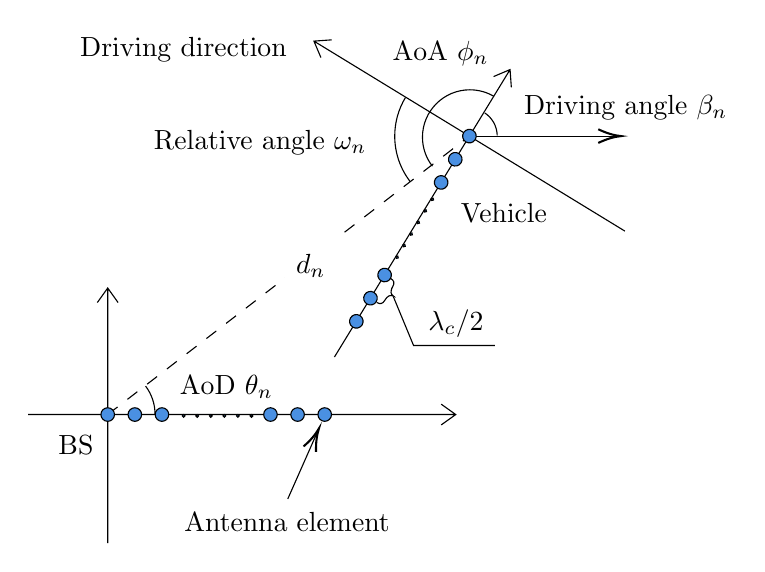
\begin{tikzpicture}[x=0.75pt,y=0.75pt,yscale=-1,xscale=1]
%uncomment if require: \path (0,400); %set diagram left start at 0, and has height of 400

%Straight Lines [id:da07907463350352173] 
\draw    (375.56,111.37) -- (446.58,111.37) ;
\draw [shift={(448.58,111.37)}, rotate = 180] [color={rgb, 255:red, 0; green, 0; blue, 0 }  ][line width=0.75]    (10.93,-3.29) .. controls (6.95,-1.4) and (3.31,-0.3) .. (0,0) .. controls (3.31,0.3) and (6.95,1.4) .. (10.93,3.29)   ;
%Straight Lines [id:da09010349521286487] 
\draw  [dash pattern={on 4.5pt off 4.5pt}]  (201.29,245.52) -- (375.56,111.37) ;
%Shape: Axis 2D [id:dp11110074206871123] 
\draw  (310.53,217.81) -- (395.14,79.32)(300.65,65.61) -- (450.47,157.14) (387.22,82.68) -- (395.14,79.32) -- (395.76,87.9) (304.01,73.53) -- (300.65,65.61) -- (309.23,64.99)  ;
%Shape: Arc [id:dp3222228343280493] 
\draw  [draw opacity=0] (357.72,125.86) .. controls (354.72,122) and (352.94,117.15) .. (352.94,111.89) .. controls (352.94,99.28) and (363.16,89.06) .. (375.76,89.06) .. controls (379.98,89.06) and (383.94,90.21) .. (387.33,92.2) -- (375.76,111.89) -- cycle ; \draw   (357.72,125.86) .. controls (354.72,122) and (352.94,117.15) .. (352.94,111.89) .. controls (352.94,99.28) and (363.16,89.06) .. (375.76,89.06) .. controls (379.98,89.06) and (383.94,90.21) .. (387.33,92.2) ;
%Shape: Ellipse [id:dp5010975008749191] 
\draw  [color={rgb, 255:red, 0; green, 0; blue, 0 }  ,draw opacity=1 ][fill={rgb, 255:red, 74; green, 144; blue, 226 }  ,fill opacity=1 ] (319.38,203.41) .. controls (317.84,202.47) and (317.35,200.45) .. (318.29,198.91) .. controls (319.23,197.37) and (321.24,196.89) .. (322.78,197.83) .. controls (324.32,198.77) and (324.81,200.78) .. (323.87,202.32) .. controls (322.93,203.86) and (320.92,204.35) .. (319.38,203.41) -- cycle ;
%Shape: Ellipse [id:dp890164411693988] 
\draw  [color={rgb, 255:red, 0; green, 0; blue, 0 }  ,draw opacity=1 ][fill={rgb, 255:red, 74; green, 144; blue, 226 }  ,fill opacity=1 ] (326.19,192.25) .. controls (324.65,191.31) and (324.16,189.3) .. (325.1,187.76) .. controls (326.04,186.22) and (328.05,185.73) .. (329.59,186.67) .. controls (331.13,187.61) and (331.62,189.62) .. (330.68,191.16) .. controls (329.74,192.7) and (327.73,193.19) .. (326.19,192.25) -- cycle ;
%Shape: Ellipse [id:dp897136838434427] 
\draw  [color={rgb, 255:red, 0; green, 0; blue, 0 }  ,draw opacity=1 ][fill={rgb, 255:red, 74; green, 144; blue, 226 }  ,fill opacity=1 ] (333,181.09) .. controls (331.46,180.15) and (330.97,178.14) .. (331.91,176.6) .. controls (332.85,175.06) and (334.86,174.58) .. (336.4,175.52) .. controls (337.94,176.46) and (338.43,178.47) .. (337.49,180.01) .. controls (336.55,181.55) and (334.54,182.03) .. (333,181.09) -- cycle ;

%Shape: Ellipse [id:dp8384533754895014] 
\draw  [color={rgb, 255:red, 0; green, 0; blue, 0 }  ,draw opacity=1 ][fill={rgb, 255:red, 74; green, 144; blue, 226 }  ,fill opacity=1 ] (360.24,136.47) .. controls (358.69,135.53) and (358.21,133.52) .. (359.15,131.98) .. controls (360.09,130.44) and (362.1,129.96) .. (363.64,130.9) .. controls (365.18,131.84) and (365.67,133.85) .. (364.73,135.39) .. controls (363.79,136.93) and (361.78,137.41) .. (360.24,136.47) -- cycle ;
%Shape: Ellipse [id:dp7475535744692714] 
\draw  [color={rgb, 255:red, 0; green, 0; blue, 0 }  ,draw opacity=1 ][fill={rgb, 255:red, 74; green, 144; blue, 226 }  ,fill opacity=1 ] (367.04,125.32) .. controls (365.5,124.38) and (365.02,122.37) .. (365.96,120.83) .. controls (366.9,119.29) and (368.91,118.8) .. (370.45,119.74) .. controls (371.99,120.68) and (372.48,122.69) .. (371.54,124.23) .. controls (370.6,125.77) and (368.58,126.26) .. (367.04,125.32) -- cycle ;
%Shape: Ellipse [id:dp004518086638926722] 
\draw  [color={rgb, 255:red, 0; green, 0; blue, 0 }  ,draw opacity=1 ][fill={rgb, 255:red, 74; green, 144; blue, 226 }  ,fill opacity=1 ] (373.85,114.16) .. controls (372.31,113.22) and (371.83,111.21) .. (372.77,109.67) .. controls (373.71,108.13) and (375.72,107.64) .. (377.26,108.59) .. controls (378.8,109.53) and (379.28,111.54) .. (378.34,113.08) .. controls (377.4,114.62) and (375.39,115.1) .. (373.85,114.16) -- cycle ;

%Shape: Ellipse [id:dp633770258342514] 
\draw  [color={rgb, 255:red, 0; green, 0; blue, 0 }  ,draw opacity=1 ][fill={rgb, 255:red, 74; green, 144; blue, 226 }  ,fill opacity=1 ] (340.37,170.28) .. controls (340.06,170.09) and (339.96,169.69) .. (340.15,169.38) .. controls (340.34,169.07) and (340.74,168.98) .. (341.05,169.16) .. controls (341.35,169.35) and (341.45,169.75) .. (341.26,170.06) .. controls (341.08,170.37) and (340.67,170.47) .. (340.37,170.28) -- cycle ;
%Shape: Ellipse [id:dp8394591104605615] 
\draw  [color={rgb, 255:red, 0; green, 0; blue, 0 }  ,draw opacity=1 ][fill={rgb, 255:red, 74; green, 144; blue, 226 }  ,fill opacity=1 ] (347.17,159.12) .. controls (346.87,158.94) and (346.77,158.53) .. (346.96,158.23) .. controls (347.15,157.92) and (347.55,157.82) .. (347.86,158.01) .. controls (348.16,158.2) and (348.26,158.6) .. (348.07,158.91) .. controls (347.88,159.22) and (347.48,159.31) .. (347.17,159.12) -- cycle ;
%Shape: Ellipse [id:dp44537030484763485] 
\draw  [color={rgb, 255:red, 0; green, 0; blue, 0 }  ,draw opacity=1 ][fill={rgb, 255:red, 74; green, 144; blue, 226 }  ,fill opacity=1 ] (353.98,147.97) .. controls (353.68,147.78) and (353.58,147.38) .. (353.77,147.07) .. controls (353.95,146.76) and (354.36,146.67) .. (354.66,146.85) .. controls (354.97,147.04) and (355.07,147.44) .. (354.88,147.75) .. controls (354.69,148.06) and (354.29,148.16) .. (353.98,147.97) -- cycle ;
%Shape: Ellipse [id:dp0254943139239715] 
\draw  [color={rgb, 255:red, 0; green, 0; blue, 0 }  ,draw opacity=1 ][fill={rgb, 255:red, 74; green, 144; blue, 226 }  ,fill opacity=1 ] (343.77,164.7) .. controls (343.46,164.51) and (343.36,164.11) .. (343.55,163.8) .. controls (343.74,163.5) and (344.14,163.4) .. (344.45,163.59) .. controls (344.76,163.77) and (344.86,164.18) .. (344.67,164.48) .. controls (344.48,164.79) and (344.08,164.89) .. (343.77,164.7) -- cycle ;
%Shape: Ellipse [id:dp49004618827916047] 
\draw  [color={rgb, 255:red, 0; green, 0; blue, 0 }  ,draw opacity=1 ][fill={rgb, 255:red, 74; green, 144; blue, 226 }  ,fill opacity=1 ] (350.58,153.55) .. controls (350.27,153.36) and (350.17,152.96) .. (350.36,152.65) .. controls (350.55,152.34) and (350.95,152.24) .. (351.26,152.43) .. controls (351.57,152.62) and (351.67,153.02) .. (351.48,153.33) .. controls (351.29,153.64) and (350.89,153.73) .. (350.58,153.55) -- cycle ;
%Shape: Ellipse [id:dp6897242875279402] 
\draw  [color={rgb, 255:red, 0; green, 0; blue, 0 }  ,draw opacity=1 ][fill={rgb, 255:red, 74; green, 144; blue, 226 }  ,fill opacity=1 ] (357.39,142.39) .. controls (357.08,142.2) and (356.98,141.8) .. (357.17,141.49) .. controls (357.36,141.19) and (357.76,141.09) .. (358.07,141.28) .. controls (358.38,141.46) and (358.47,141.87) .. (358.29,142.17) .. controls (358.1,142.48) and (357.7,142.58) .. (357.39,142.39) -- cycle ;


%Shape: Arc [id:dp3331329274593001] 
\draw  [draw opacity=0] (347.08,133.37) .. controls (342.38,127.28) and (339.58,119.66) .. (339.58,111.37) .. controls (339.58,104.58) and (341.46,98.22) .. (344.74,92.8) -- (375.56,111.37) -- cycle ; \draw   (347.08,133.37) .. controls (342.38,127.28) and (339.58,119.66) .. (339.58,111.37) .. controls (339.58,104.58) and (341.46,98.22) .. (344.74,92.8) ;
%Shape: Axis 2D [id:dp6630697678007663] 
\draw  (163,245.52) -- (368.97,245.52)(201.29,184.56) -- (201.29,307.46) (361.97,240.52) -- (368.97,245.52) -- (361.97,250.52) (196.29,191.56) -- (201.29,184.56) -- (206.29,191.56)  ;
%Shape: Arc [id:dp8032341000802897] 
\draw  [draw opacity=0] (219.55,231.82) .. controls (222.42,235.64) and (224.11,240.38) .. (224.11,245.52) .. controls (224.11,245.52) and (224.11,245.53) .. (224.11,245.53) -- (201.29,245.52) -- cycle ; \draw   (219.55,231.82) .. controls (222.42,235.64) and (224.11,240.38) .. (224.11,245.52) .. controls (224.11,245.52) and (224.11,245.53) .. (224.11,245.53) ;
%Shape: Ellipse [id:dp18925787396184124] 
\draw  [color={rgb, 255:red, 0; green, 0; blue, 0 }  ,draw opacity=1 ][fill={rgb, 255:red, 74; green, 144; blue, 226 }  ,fill opacity=1 ] (198.02,245.52) .. controls (198.02,243.72) and (199.48,242.25) .. (201.29,242.25) .. controls (203.09,242.25) and (204.56,243.72) .. (204.56,245.52) .. controls (204.56,247.32) and (203.09,248.79) .. (201.29,248.79) .. controls (199.48,248.79) and (198.02,247.32) .. (198.02,245.52) -- cycle ;
%Shape: Ellipse [id:dp04884015005212705] 
\draw  [color={rgb, 255:red, 0; green, 0; blue, 0 }  ,draw opacity=1 ][fill={rgb, 255:red, 74; green, 144; blue, 226 }  ,fill opacity=1 ] (211.09,245.52) .. controls (211.09,243.72) and (212.55,242.25) .. (214.36,242.25) .. controls (216.16,242.25) and (217.63,243.72) .. (217.63,245.52) .. controls (217.63,247.32) and (216.16,248.79) .. (214.36,248.79) .. controls (212.55,248.79) and (211.09,247.32) .. (211.09,245.52) -- cycle ;
%Shape: Ellipse [id:dp5732317293589196] 
\draw  [color={rgb, 255:red, 0; green, 0; blue, 0 }  ,draw opacity=1 ][fill={rgb, 255:red, 74; green, 144; blue, 226 }  ,fill opacity=1 ] (224.16,245.52) .. controls (224.16,243.72) and (225.62,242.25) .. (227.43,242.25) .. controls (229.23,242.25) and (230.7,243.72) .. (230.7,245.52) .. controls (230.7,247.32) and (229.23,248.79) .. (227.43,248.79) .. controls (225.62,248.79) and (224.16,247.32) .. (224.16,245.52) -- cycle ;

%Shape: Ellipse [id:dp41070623189345956] 
\draw  [color={rgb, 255:red, 0; green, 0; blue, 0 }  ,draw opacity=1 ][fill={rgb, 255:red, 74; green, 144; blue, 226 }  ,fill opacity=1 ] (276.44,245.52) .. controls (276.44,243.72) and (277.9,242.25) .. (279.71,242.25) .. controls (281.51,242.25) and (282.97,243.72) .. (282.97,245.52) .. controls (282.97,247.32) and (281.51,248.79) .. (279.71,248.79) .. controls (277.9,248.79) and (276.44,247.32) .. (276.44,245.52) -- cycle ;
%Shape: Ellipse [id:dp8237774927897598] 
\draw  [color={rgb, 255:red, 0; green, 0; blue, 0 }  ,draw opacity=1 ][fill={rgb, 255:red, 74; green, 144; blue, 226 }  ,fill opacity=1 ] (289.51,245.52) .. controls (289.51,243.72) and (290.97,242.25) .. (292.77,242.25) .. controls (294.58,242.25) and (296.04,243.72) .. (296.04,245.52) .. controls (296.04,247.32) and (294.58,248.79) .. (292.77,248.79) .. controls (290.97,248.79) and (289.51,247.32) .. (289.51,245.52) -- cycle ;
%Shape: Ellipse [id:dp036366987423380515] 
\draw  [color={rgb, 255:red, 0; green, 0; blue, 0 }  ,draw opacity=1 ][fill={rgb, 255:red, 74; green, 144; blue, 226 }  ,fill opacity=1 ] (302.58,245.52) .. controls (302.58,243.72) and (304.04,242.25) .. (305.84,242.25) .. controls (307.65,242.25) and (309.11,243.72) .. (309.11,245.52) .. controls (309.11,247.32) and (307.65,248.79) .. (305.84,248.79) .. controls (304.04,248.79) and (302.58,247.32) .. (302.58,245.52) -- cycle ;

%Shape: Ellipse [id:dp1962117770084869] 
\draw  [color={rgb, 255:red, 0; green, 0; blue, 0 }  ,draw opacity=1 ][fill={rgb, 255:red, 74; green, 144; blue, 226 }  ,fill opacity=1 ] (237.23,246.17) .. controls (237.23,245.81) and (237.52,245.52) .. (237.88,245.52) .. controls (238.24,245.52) and (238.54,245.81) .. (238.54,246.17) .. controls (238.54,246.53) and (238.24,246.83) .. (237.88,246.83) .. controls (237.52,246.83) and (237.23,246.53) .. (237.23,246.17) -- cycle ;
%Shape: Ellipse [id:dp18231164623431284] 
\draw  [color={rgb, 255:red, 0; green, 0; blue, 0 }  ,draw opacity=1 ][fill={rgb, 255:red, 74; green, 144; blue, 226 }  ,fill opacity=1 ] (250.3,246.17) .. controls (250.3,245.81) and (250.59,245.52) .. (250.95,245.52) .. controls (251.31,245.52) and (251.61,245.81) .. (251.61,246.17) .. controls (251.61,246.53) and (251.31,246.83) .. (250.95,246.83) .. controls (250.59,246.83) and (250.3,246.53) .. (250.3,246.17) -- cycle ;
%Shape: Ellipse [id:dp8670442515261287] 
\draw  [color={rgb, 255:red, 0; green, 0; blue, 0 }  ,draw opacity=1 ][fill={rgb, 255:red, 74; green, 144; blue, 226 }  ,fill opacity=1 ] (263.37,246.17) .. controls (263.37,245.81) and (263.66,245.52) .. (264.02,245.52) .. controls (264.38,245.52) and (264.68,245.81) .. (264.68,246.17) .. controls (264.68,246.53) and (264.38,246.83) .. (264.02,246.83) .. controls (263.66,246.83) and (263.37,246.53) .. (263.37,246.17) -- cycle ;
%Shape: Ellipse [id:dp8145801535707166] 
\draw  [color={rgb, 255:red, 0; green, 0; blue, 0 }  ,draw opacity=1 ][fill={rgb, 255:red, 74; green, 144; blue, 226 }  ,fill opacity=1 ] (243.76,246.17) .. controls (243.76,245.81) and (244.06,245.52) .. (244.42,245.52) .. controls (244.78,245.52) and (245.07,245.81) .. (245.07,246.17) .. controls (245.07,246.53) and (244.78,246.83) .. (244.42,246.83) .. controls (244.06,246.83) and (243.76,246.53) .. (243.76,246.17) -- cycle ;
%Shape: Ellipse [id:dp10370964786130055] 
\draw  [color={rgb, 255:red, 0; green, 0; blue, 0 }  ,draw opacity=1 ][fill={rgb, 255:red, 74; green, 144; blue, 226 }  ,fill opacity=1 ] (256.83,246.17) .. controls (256.83,245.81) and (257.13,245.52) .. (257.49,245.52) .. controls (257.85,245.52) and (258.14,245.81) .. (258.14,246.17) .. controls (258.14,246.53) and (257.85,246.83) .. (257.49,246.83) .. controls (257.13,246.83) and (256.83,246.53) .. (256.83,246.17) -- cycle ;
%Shape: Ellipse [id:dp6317400721278357] 
\draw  [color={rgb, 255:red, 0; green, 0; blue, 0 }  ,draw opacity=1 ][fill={rgb, 255:red, 74; green, 144; blue, 226 }  ,fill opacity=1 ] (269.9,246.17) .. controls (269.9,245.81) and (270.2,245.52) .. (270.56,245.52) .. controls (270.92,245.52) and (271.21,245.81) .. (271.21,246.17) .. controls (271.21,246.53) and (270.92,246.83) .. (270.56,246.83) .. controls (270.2,246.83) and (269.9,246.53) .. (269.9,246.17) -- cycle ;


%Straight Lines [id:da2733690085480769] 
\draw    (288.04,286.2) -- (302.26,254.05) ;
\draw [shift={(303.07,252.22)}, rotate = 473.86] [color={rgb, 255:red, 0; green, 0; blue, 0 }  ][line width=0.75]    (10.93,-3.29) .. controls (6.95,-1.4) and (3.31,-0.3) .. (0,0) .. controls (3.31,0.3) and (6.95,1.4) .. (10.93,3.29)   ;
%Shape: Brace [id:dp14470849407683806] 
\draw   (330.98,191.56) .. controls (332.57,192.48) and (333.82,192.15) .. (334.74,190.56) -- (334.74,190.56) .. controls (336.05,188.29) and (337.49,187.62) .. (339.08,188.53) .. controls (337.49,187.62) and (337.36,186.03) .. (338.67,183.76)(338.08,184.78) -- (338.67,183.76) .. controls (339.59,182.17) and (339.26,180.92) .. (337.67,180) ;
%Straight Lines [id:da5070089969356341] 
\draw    (338.98,188.89) -- (348.64,212.23) -- (387.86,212.23) ;
%Shape: Arc [id:dp6163818800344831] 
\draw  [draw opacity=0] (382.98,100.22) .. controls (386.49,102.56) and (388.83,106.51) .. (388.95,111.01) -- (375.56,111.37) -- cycle ; \draw   (382.98,100.22) .. controls (386.49,102.56) and (388.83,106.51) .. (388.95,111.01) ;

% Text Node
\draw  [draw opacity=0][fill={rgb, 255:red, 255; green, 255; blue, 255 }  ,fill opacity=1 ]  (286.63,160.79) -- (311.63,160.79) -- (311.63,186.79) -- (286.63,186.79) -- cycle  ;
\draw (299.13,173.79) node    {$d_{n}$};
% Text Node
\draw (369.06,201.76) node    {$\lambda _{c} /2$};
% Text Node
\draw (392.19,148.4) node   [align=left] {Vehicle};
% Text Node
\draw (287.71,297.4) node   [align=left] {Antenna element};
% Text Node
\draw (186.01,260.4) node   [align=left] {BS};
% Text Node
\draw (237.77,69.5) node   [align=left] {Driving direction};
% Text Node
\draw (258.5,232) node   [align=left] {AoD $\displaystyle \theta _{n}$};
% Text Node
\draw (361.68,71.5) node   [align=left] {AoA $\displaystyle \phi _{n}$};
% Text Node
\draw (450.87,97.5) node   [align=left] {Driving angle $\displaystyle \beta _{n}$};
% Text Node
\draw (274.77,114.5) node   [align=left] {Relative angle $\displaystyle \omega _{n}$};


\end{tikzpicture}}
    \caption{Channel geometry}
    \label{geo}
\end{figure}

% 场景和天线数
A mmWave vehicular communication scenario including a vehicle with $M_r$ antenna elements and a BS with $M_t$ antenna elements is considered, as shown in Fig.~\ref{geo}.
% 天线结构、阵元间距、赋形技术
Both of them are equipped with a single RF chain and uniform linear array (ULA) of half-wave interval antenna.
Analog beamforming based on quantized phase shifter is adopted at both BS and vehicle. 

% 信道模型
The Saleh-Valenzuela channel model is taken as channel model in this paper.
The definitions of channel parameters refer to $28$ GHz model \cite{Akdeniz2014}, which are derived by real experimental data measured in New York City.
And only the case of single cluster under LOS condition is considered in this paper.
The narrowband time-varying $L$ subpaths channel matrix between the vehicle and BS at $n$th time step is $\mathbf{H}_{n} \in \mathbb{C}^{M_{r} \times M_{t}}$, which is given as:
\begin{equation}
    \mathbf{H}_{n} =\sqrt{\frac{M_r M_t}{L}} \sum\limits ^{L}_{l=1} g_{ln}\mathbf{a}_{r}( \phi _{ln})\mathbf{a}^{H}_{t}( \theta _{ln})
    \label{cm}
\end{equation}
where $g_{ln} \in \mathbb{C}$ is complex fading gain on subpath $l$, $\phi_{ln}$ and $\theta_{ln}$ are the AoA and AoD of the $l$th subpath, respectively. 
$\phi_{ln} = \phi_n + \Delta \phi_{ln}$ and $\theta _{ln} =\theta _{n} +\Delta \theta _{ln}$, where $\phi_{n}$ and $\theta_{n}$ is the AoA and AoD of the cluster center, $\Delta \phi _{ln} \sim \mathcal{WN}( \delta ^{2}_{rn})$, $\Delta \theta _{ln} \sim \mathcal{WN}( \delta ^{2}_{tn})$, $\delta_{tn} \sim \mathcal{E}(\lambda_t)$ and $\delta_{rn} \sim \mathcal{E}(\lambda_r)$.
$\lambda_t$ and $\lambda_r$ are root-mean-square (RMS) angular spread of transmitter and receiver, respectively.
Note that the cluster angles depend on the geometric position of the vehicle and the BS.
The complex fading gain on $l$th subpath at $n$th time step is given by:
\begin{equation}
    g_{ln} =\overline{g}_{ln} e^{j2\pi t_{n} f_{Dn,max} cos( \omega _{ln})}, \overline{g}_{ln} \sim \mathcal{CN}\left( 0, 10^{-0.1PL_n}\right)
    \label{ssfg}
\end{equation}
where $t_{n}$ is the signal transmission time, $f_{Dn,max} ={v_{n}}/{\lambda _{c}}$ is maximum Doppler shift, $v_{n}$ is the speed of vehicle, $\lambda _{c}$ is the carrier wavelength, $\omega _{ln} = \phi_{ln} - \pi / 2$ is the AoA of subpath $l$ relative to the direction of vehicle, and $PL_n$ is omnidirectional path loss at time step $n$, which is defined as:
\begin{equation}
    PL_n = 61.4 + 20 \log(d_n) + \xi~[dB]
    \label{pl}
\end{equation}
where $d_n$ is distance between the vehicle and the BS, and $\xi \sim \mathcal{N}(0, \sigma_p^2)$.
% 阵列响应矢量
The array response vector of ULA with $M$ half-wave interval antenna elements is given by:
\begin{equation}
    \mathbf{a}( M,\varphi ) =\frac{1}{\sqrt{M}}\left[ 1,e^{j\pi cos( \varphi )} ,...,e^{j\pi ( M-1) cos( \varphi )}\right]^{T}
    \label{arv}
\end{equation}
where $\varphi$ is the arrival angle of the signal. When AoA of the vehicle is $\phi$ and AoD of the BS is $\theta$, the array response vectors of both are $\mathbf{a}_{r}( \phi ) =\mathbf{a}( M_{r} ,\phi )$ and $\mathbf{a}_{t}( \theta ) =\mathbf{a}( M_{t} ,\theta )$, respectively.

% 管理方式
Beam management procedure is as follows. The reference signals are sent to the vehicle from the BS, the vehicle measures and determines the optimal beam pair for communication, then feeds back to the BS.

% 码本设计
A discrete resolution $b$-bit codebook is adopted to perform beam search, where $b$ is the number of bits for quantized phase shifters.
For a $b$-bit codebook, it is consisted of $2^b$ beam patterns.
In this paper, $b$ is assumed to be $log_2{2M}$ for a terminal with $M$ antennas.
The candidate beam angles vector $\mathbf{b}_{M}$ for the terminal is given by:
% $b$ is assumed to be $2log_2 M$ for a $M$-element antenna terminal, and the candidate beam angles vector $\mathbf{b}_M$ is given by:
\begin{equation}
    \mathbf{b}_{M} = \left[\frac{1}{2M}\pi, \frac{2}{2M}\pi, ..., \frac{2M-1}{2M}\pi, \pi\right]^T
\end{equation}
Thus, there are $2M_r$ beam patterns for the vehicle, and $2M_t$ beam patterns for the BS, and the beam codebooks of the vehicle and the BS are:
% Note that another codebook which achieves uniform maximum gain in all direction is not used for this scheme, due to its low spatial resolution near $0$ and $\pi$ resulting in network underfitting.
% The beam codebooks of the vehicle and the BS are:
\begin{gather}
    \begin{aligned}
        \mathbf{W} =&\left[\mathbf{a}_{r}([\mathbf{b}_{M_r}]_1) ,\mathbf{a}_{r}\left([\mathbf{b}_{M_r}]_2 \right) ,...,\mathbf{a}_{r}\left([\mathbf{b}_{M_r}]_{2M_r} \right)\right] \\
        \mathbf{F} =&\left[\mathbf{a}_{t}([\mathbf{b}_{M_t}]_1) ,\mathbf{a}_{t}\left([\mathbf{b}_{M_t}]_2 \right) ,...,\mathbf{a}_{t}\left([\mathbf{b}_{M_t}]_{2M_t} \right)\right]
    \end{aligned}
\end{gather}
where $\mathbf{W} \in \mathbb{C}^{M_{r} \times 2M_r}$ is the codebook of vehicle, and $\mathbf{F} \in \mathbb{C}^{M_{t} \times 2M_t}$ is the codebook of BS. Each column vector of the codebook is codeword which represents a beam pattern, each entry in the column is phase rotation for corresponding antenna element to generate directional beam.

% 接收信号
At time step $n$, for transmitted signal $x_n$ from the BS, received signal $y_n$ at the vehicle is given by:
\begin{equation}
    y_n = \mathbf{w}^H_n \mathbf{H}_n \mathbf{f}_n x_n + \mathbf{w}^H_n \mathbf{v}_n
    \label{rs}
\end{equation}
where $\mathbf{w}_n$ and $\mathbf{f}_n$ are combining and beamforming vector, which are the codeword in $\mathbf{W}$ and $\mathbf{F}$, respectively.
$\mathbf{v}_n$ is Gaussian noise and $\mathbf{v}_n \sim \mathcal{CN}(0, \sigma^2_v \mathbf{I}_{M_r})$. 

\begin{figure*}[ht]
    \centerline{\includegraphics[scale=1]{procedure.pdf}}
    \caption{Procedure of FC-BET scheme}
    \label{procedure}
\end{figure*}

\section{Fast Consecutive Beam Tracking Scheme}\label{LBTS}

% 网络
\subsection{The LSTM Network}

% 问题定义
The purpose of beam tracking is to obtain optimal beam angles with as few beam measurements as possible for reducing the overhead brought by beam training.
Since the vehicle must travel in a particular direction on the road and the mmWave beams are correlated with the position of vehicles \cite{Aviles2016, Wang2019}, the problem of beam tracking can be formulated as a time series regression problem.

\begin{figure}[!b]
    \centerline{

\tikzset{every picture/.style={line width=0.75pt}} %set default line width to 0.75pt        

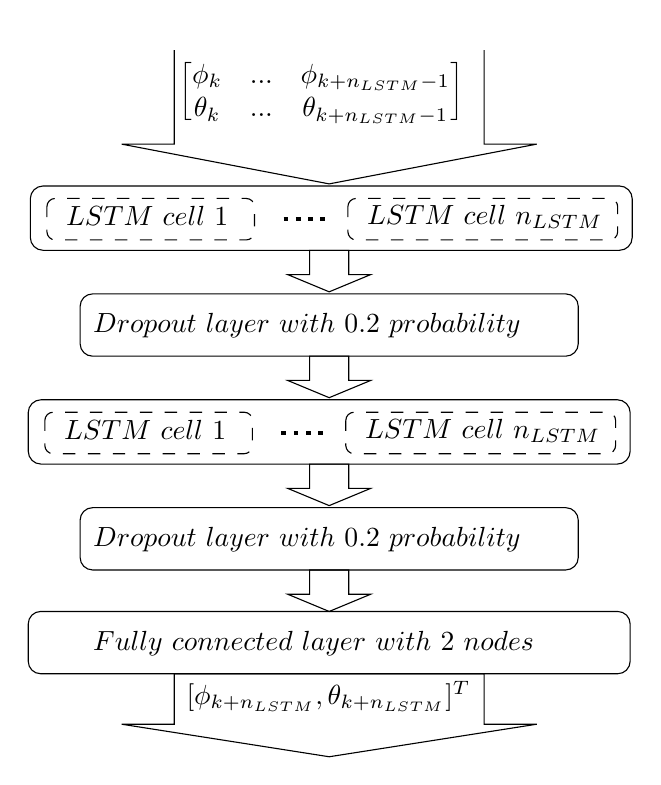
\begin{tikzpicture}[x=0.75pt,y=0.75pt,yscale=-1,xscale=1]
%uncomment if require: \path (0,631); %set diagram left start at 0, and has height of 631

%Rounded Rect [id:dp8311889338813093] 
\draw   (186,225.8) .. controls (186,229.22) and (188.78,232) .. (192.2,232) -- (469.8,232) .. controls (473.22,232) and (476,229.22) .. (476,225.8) -- (476,207.2) .. controls (476,203.78) and (473.22,201) .. (469.8,201) -- (192.2,201) .. controls (188.78,201) and (186,203.78) .. (186,207.2) -- cycle ;
%Rounded Rect [id:dp8257681201044845] 
\draw  [dash pattern={on 4.5pt off 4.5pt}] (194,211) .. controls (194,208.79) and (195.79,207) .. (198,207) -- (290,207) .. controls (292.21,207) and (294,208.79) .. (294,211) -- (294,223) .. controls (294,225.21) and (292.21,227) .. (290,227) -- (198,227) .. controls (195.79,227) and (194,225.21) .. (194,223) -- cycle ;

%Rounded Rect [id:dp9335045318672898] 
\draw  [dash pattern={on 4.5pt off 4.5pt}] (339,211) .. controls (339,208.79) and (340.79,207) .. (343,207) -- (465,207) .. controls (467.21,207) and (469,208.79) .. (469,211) -- (469,223) .. controls (469,225.21) and (467.21,227) .. (465,227) -- (343,227) .. controls (340.79,227) and (339,225.21) .. (339,223) -- cycle ;

%Straight Lines [id:da4456092694713579] 
\draw [line width=1.5]  [dash pattern={on 1.69pt off 2.76pt}]  (308,217) -- (330,217) ;

%Rounded Rect [id:dp8578025625259913] 
\draw  [fill={rgb, 255:red, 255; green, 255; blue, 255 }  ,fill opacity=1 ] (185,430) .. controls (185,433.31) and (187.69,436) .. (191,436) -- (469,436) .. controls (472.31,436) and (475,433.31) .. (475,430) -- (475,412) .. controls (475,408.69) and (472.31,406) .. (469,406) -- (191,406) .. controls (187.69,406) and (185,408.69) .. (185,412) -- cycle ;
%Rounded Rect [id:dp6298572435990919] 
\draw   (210,277) .. controls (210,280.31) and (212.69,283) .. (216,283) -- (444,283) .. controls (447.31,283) and (450,280.31) .. (450,277) -- (450,259) .. controls (450,255.69) and (447.31,253) .. (444,253) -- (216,253) .. controls (212.69,253) and (210,255.69) .. (210,259) -- cycle ;

%Rounded Rect [id:dp21646877110312346] 
\draw   (210,380) .. controls (210,383.31) and (212.69,386) .. (216,386) -- (444,386) .. controls (447.31,386) and (450,383.31) .. (450,380) -- (450,362) .. controls (450,358.69) and (447.31,356) .. (444,356) -- (216,356) .. controls (212.69,356) and (210,358.69) .. (210,362) -- cycle ;

%Down Arrow [id:dp009213193607987225] 
\draw   (310,346.69) -- (320.58,346.69) -- (320.58,335) -- (339.42,335) -- (339.42,346.69) -- (350,346.69) -- (330,355) -- cycle ;
%Down Arrow [id:dp5633595669822283] 
\draw   (230,180.84) -- (255.33,180.84) -- (255.33,130) -- (404.67,130) -- (404.67,180.84) -- (430,180.84) -- (330,200) -- cycle ;
%Flowchart: Process [id:dp7387059282658188] 
\draw  [color={rgb, 255:red, 255; green, 255; blue, 255 }  ,draw opacity=1 ][fill={rgb, 255:red, 255; green, 255; blue, 255 }  ,fill opacity=1 ] (246,125) -- (426,125) -- (426,135) -- (246,135) -- cycle ;
%Down Arrow [id:dp9615271374443121] 
\draw   (230,460.32) -- (255.33,460.32) -- (255.33,436) -- (404.67,436) -- (404.67,460.32) -- (430,460.32) -- (330,476) -- cycle ;
%Down Arrow [id:dp2799951517638246] 
\draw   (310,397.69) -- (320.58,397.69) -- (320.58,386) -- (339.42,386) -- (339.42,397.69) -- (350,397.69) -- (330,406) -- cycle ;
%Down Arrow [id:dp8337941309291784] 
\draw   (310,294.69) -- (320.58,294.69) -- (320.58,283) -- (339.42,283) -- (339.42,294.69) -- (350,294.69) -- (330,303) -- cycle ;
%Down Arrow [id:dp5272716984374778] 
\draw   (310,243.69) -- (320.58,243.69) -- (320.58,232) -- (339.42,232) -- (339.42,243.69) -- (350,243.69) -- (330,252) -- cycle ;
%Rounded Rect [id:dp40089685674424747] 
\draw   (185,328.8) .. controls (185,332.22) and (187.78,335) .. (191.2,335) -- (468.8,335) .. controls (472.22,335) and (475,332.22) .. (475,328.8) -- (475,310.2) .. controls (475,306.78) and (472.22,304) .. (468.8,304) -- (191.2,304) .. controls (187.78,304) and (185,306.78) .. (185,310.2) -- cycle ;
%Rounded Rect [id:dp407581701253965] 
\draw  [dash pattern={on 4.5pt off 4.5pt}] (193,314) .. controls (193,311.79) and (194.79,310) .. (197,310) -- (289,310) .. controls (291.21,310) and (293,311.79) .. (293,314) -- (293,326) .. controls (293,328.21) and (291.21,330) .. (289,330) -- (197,330) .. controls (194.79,330) and (193,328.21) .. (193,326) -- cycle ;

%Rounded Rect [id:dp025623893665189357] 
\draw  [dash pattern={on 4.5pt off 4.5pt}] (338,314) .. controls (338,311.79) and (339.79,310) .. (342,310) -- (464,310) .. controls (466.21,310) and (468,311.79) .. (468,314) -- (468,326) .. controls (468,328.21) and (466.21,330) .. (464,330) -- (342,330) .. controls (339.79,330) and (338,328.21) .. (338,326) -- cycle ;

%Straight Lines [id:da4692192638928624] 
\draw [line width=1.5]  [dash pattern={on 1.69pt off 2.76pt}]  (307,320) -- (329,320) ;


% Text Node
\draw (202,209.43) node [anchor=north west][inner sep=0.75pt]    {$LSTM\ cell\ 1$};
% Text Node
\draw (347,208.93) node [anchor=north west][inner sep=0.75pt]    {$LSTM\ cell\ n_{LSTM}$};
% Text Node
\draw (256,139.26) node [anchor=north west][inner sep=0.75pt]    {$\begin{bmatrix}
\phi _{k} & ... & \phi _{k+n_{LSTM} -1}\\
\theta _{k} & ... & \theta _{k+n_{LSTM} -1}
\end{bmatrix}$};
% Text Node
\draw (215,414.06) node [anchor=north west][inner sep=0.75pt]    {$Fully\ connected\ layer\ with\ 2\ nodes$};
% Text Node
\draw (215,364.06) node [anchor=north west][inner sep=0.75pt]    {$Dropout\ layer\ with\ 0.2\ probability$};
% Text Node
\draw (260,438.26) node [anchor=north west][inner sep=0.75pt]    {$[ \phi _{k+n_{LSTM}} ,\theta _{k+n_{LSTM}}]^{T}$};
% Text Node
\draw (215,261.06) node [anchor=north west][inner sep=0.75pt]    {$Dropout\ layer\ with\ 0.2\ probability$};
% Text Node
\draw (346,311.93) node [anchor=north west][inner sep=0.75pt]    {$LSTM\ cell\ n_{LSTM}$};
% Text Node
\draw (201,312.43) node [anchor=north west][inner sep=0.75pt]    {$LSTM\ cell\ 1$};


\end{tikzpicture}}
    \caption{Structure of network}
    \label{lstm}
\end{figure}

% 结构
An artificial neural network based on LSTM is used to solve this regression problem.
LSTM has been implemented successfully in several fields such as machine translation, image captioning, speech recognition, and even stock prices prediction in economy.
It is powerful for handling time series data and learning long-term relations between features, relying on three gates, i.e. forget, input and output gates composed of neural networks (NNs) in LSTM cells.

Fig.~\ref{lstm} shows the structure of the network, which is a sequential model comprises two LSTM layers with 50 hidden units, two dropout layers with 0.2 probability and a fully connected layer with 2 nodes.
The output of the first LSTM layer is a sequence of length $n_L$, which is used as the input of the second LSTM layer.
And two dropout layers are set to prevent overfitting. 

% 损失函数?
\subsection{Loss Function}

Mean Square Error (MSE) is the most commonly used regression loss function for quantifying the error of prediction.
In \cite{Burghal2019}, considering the problem of angle ambiguity due to the periodicity of the beam angle results in unnecessary loss for large difference of beam angle when used MSE, D. Burghal et al. proposed to use a shifted cosine function as the loss function. 
However, when using this loss function, the training process may be unstable due to the multiple global minima, and the responses may not converge in a reasonable interval.
Therefore, to avoid the problem of angle ambiguity, the AoAs and AoDs are converted to interval $(0, \pi]$ before training, considering the symmetry of the cosine function around $\pi$.

% \begin{figure}[!t]
%     \centering
%     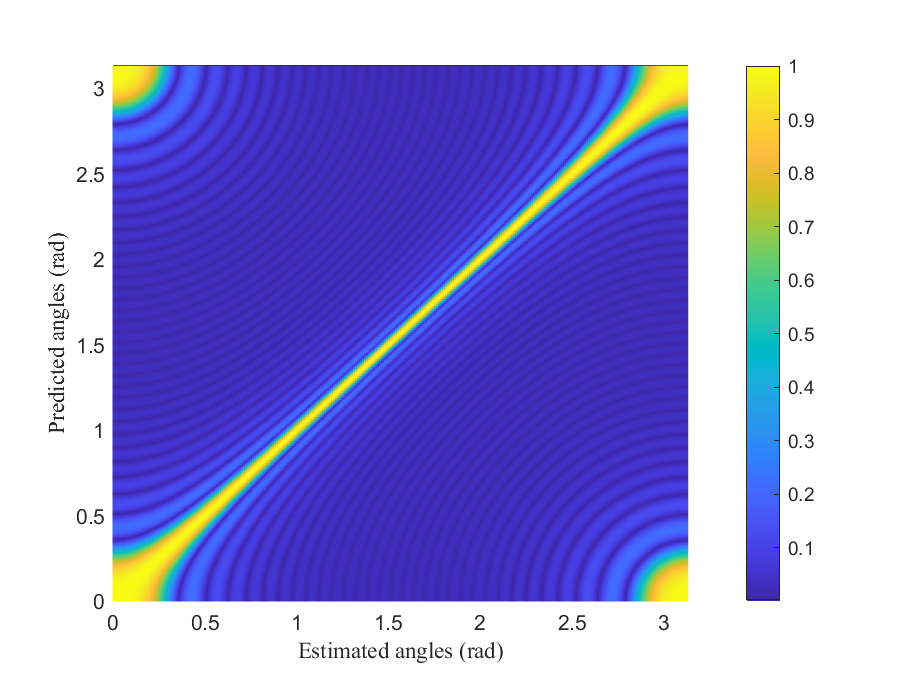
\includegraphics[scale=0.59]{results_gain}
%     \caption{Heatmap of $|\mathbf{a}^{H}(16, \theta^e)\mathbf{a}(16, \theta^p)|$}
%     \label{results_gain}
% \end{figure}

% In addition, another problem is that the codewords whose beam angle near $0$ or $\pi$ have close gains at two different angles, resulting in unnecessary loss in some cases, as shown in Fig.~\ref{results_gain}.
% For instance, in the case of the codeword whose beam angle is $\pi$, there are same gains at $0$ and $\pi$. 
% The loss should be small, even zero, if estimated angle is $0$ and predicted angle is $\pi$, although the absolute difference of them is $\pi$.
% A straightforward idea is taking $1-|\mathbf{a}^{H}(M, \theta^e)\mathbf{a}(M, \theta^p)|$ as the loss.
% Calculating this loss, however, requires array response vectors of estimated and predicted angles at the corresponding time step, which will increase the computational cost when training network.

Besides, the loss introduced by angular error should be higher as the number of corresponding antennas gets bigger, because large number of antennas leads to a narrow beam.
And the narrower the beam, the greater the effect on performance when the beam deflects.
Hence, for the AoA and AoD errors, each is multiply by a weight which depends on the number of antennas to balance this effect.

A modified MSE is used as loss function, which is defined as:
\begin{equation}
    L(\bm{\phi}, \bm{\theta}, \mathbf{M}) = \frac{\sum_{i=1}^{N}\left[M_r(\phi^{p}_{i} - \phi^{e}_{i})^2 + M_t (\theta^{p}_{i} - \theta^{e}_{i})^2\right]}{N(M_r + M_t)}
    \label{lf}
\end{equation}
where $N$ is the number of training samples, $\phi ^{e}_{i}$, $\theta ^{e}_{i}$, $\phi ^{p}_{i}$, $\theta ^{p}_{i}$, are the estimated AoA, estimated AoD, predicted AoA, and predicted AoD, respectively, for training sample $i$.

% 预测过程
\subsection{Procedure of FC-BET Scheme}

Fig.~\ref{procedure} demonstrates the procedure of FC-BET scheme.
Before exploiting the LSTM network for beam tracking, processor at the BS demands to collect historical optimal AoAs and AoDs, which are estimated by the vehicle using exhaustive beam search, to build a dataset for training the LSTM network.
The dataset is consisted of time series AoAs and AoDs of the vehicle from initial access to disconnection.
During training, the network takes the AoAs and AoDs from time step $k - n_L$ to $k - 1$ as features and the AoA and AoD at time step $k$ as responses.

After the LSTM network has been trained, the vehicle takes exhaustive beam search in consecutive $n_L$ time steps to obtain initial estimated AoAs and AoDs at the beginning of a round of beam tracking. 
The network will take the initial estimated AoAs and AoDs to predict AoA and AoD at next time step. 
Then, the predicted AoA and AoD will be used to compose new feature with the last $n_L - 1$ AoAs and AoDs in last feature.

Once the predicted AoA and AoD are obtained, the codewords whose steering angle closest to the predicted beam angles will be taken as beamforming and combining vectors.
For every time step, signal-to-noise ratio (SNR) under current prediction will be calculated and compared with a threshold ${SNR}_T$.
The network will repeat to use predicted result to compose new features to predict AoA and AoD at next time step, when the calculated SNR is greater than ${SNR}_T$.
Otherwise, a new round of estimation and prediction will be executed.
% It makes more sense to take the SNR of received signal rather than the absolute difference between predicted and estimated angles as a threshold, because there is no way to obtain a precise beam angle for judgment until it is accurately measured or predicted.

\section{Dataset Built}\label{DG}

% 信道矩阵
\subsection{Channel Matrix}

\begin{figure}[!b]
    \centerline{

% Gradient Info
  
\tikzset {_ec7nzqwik/.code = {\pgfsetadditionalshadetransform{ \pgftransformshift{\pgfpoint{0 bp } { 0 bp }  }  \pgftransformrotate{-265 }  \pgftransformscale{2 }  }}}
\pgfdeclarehorizontalshading{_xyfuj5rm5}{150bp}{rgb(0bp)=(1,1,1);
rgb(37.5bp)=(1,1,1);
rgb(62.5bp)=(0.29,0.56,0.89);
rgb(100bp)=(0.29,0.56,0.89)}

% Gradient Info
  
\tikzset {_rjiyvzeb0/.code = {\pgfsetadditionalshadetransform{ \pgftransformshift{\pgfpoint{0 bp } { 0 bp }  }  \pgftransformrotate{-73 }  \pgftransformscale{2 }  }}}
\pgfdeclarehorizontalshading{_f7g2os25i}{150bp}{rgb(0bp)=(1,1,1);
rgb(37.5bp)=(1,1,1);
rgb(62.5bp)=(0.29,0.56,0.89);
rgb(100bp)=(0.29,0.56,0.89)}
\tikzset{every picture/.style={line width=0.75pt}} %set default line width to 0.75pt        

\begin{tikzpicture}[x=0.75pt,y=0.75pt,yscale=-1,xscale=1]
%uncomment if require: \path (0,389); %set diagram left start at 0, and has height of 389

%Shape: Path Data [id:dp9439264762383368] 
\draw  [color={rgb, 255:red, 245; green, 166; blue, 35 }  ,draw opacity=1 ][fill={rgb, 255:red, 156; green, 156; blue, 156 }  ,fill opacity=1 ] (425.26,116.06) -- (425.11,116.06) -- (425.11,319.23) -- (418.05,319.23) -- (418.05,116.12) -- (417.9,116.12) .. controls (417.81,105.52) and (409.19,96.94) .. (398.56,96.94) -- (398.56,96.98) -- (195.32,96.98) -- (195.32,89.43) -- (398.56,89.43) -- (398.56,89.58) .. controls (413.23,89.58) and (425.14,101.42) .. (425.26,116.06) -- cycle ;
%Shape: Axis 2D [id:dp06192362645207816] 
\draw  (194.94,319.23) -- (459.58,319.23)(194.94,54.59) -- (194.94,319.23) -- cycle (452.58,314.23) -- (459.58,319.23) -- (452.58,324.23) (189.94,61.59) -- (194.94,54.59) -- (199.94,61.59)  ;
%Shape: Ellipse [id:dp6223646892502144] 
\draw  [fill={rgb, 255:red, 126; green, 211; blue, 33 }  ,fill opacity=1 ] (398.42,113.29) .. controls (398.42,111.31) and (400.03,109.71) .. (402.01,109.71) .. controls (403.99,109.71) and (405.6,111.31) .. (405.6,113.29) .. controls (405.6,115.27) and (403.99,116.88) .. (402.01,116.88) .. controls (400.03,116.88) and (398.42,115.27) .. (398.42,113.29) -- cycle ;
%Straight Lines [id:da38619721366461013] 
\draw    (379.17,129.34) -- (395.28,118.03) ;
\draw [shift={(396.91,116.88)}, rotate = 504.93] [color={rgb, 255:red, 0; green, 0; blue, 0 }  ][line width=0.75]    (10.93,-3.29) .. controls (6.95,-1.4) and (3.31,-0.3) .. (0,0) .. controls (3.31,0.3) and (6.95,1.4) .. (10.93,3.29)   ;
%Straight Lines [id:da15022537128136448] 
\draw    (379.55,293.56) -- (412.44,307.74) ;
\draw [shift={(414.28,308.53)}, rotate = 203.32] [color={rgb, 255:red, 0; green, 0; blue, 0 }  ][line width=0.75]    (10.93,-3.29) .. controls (6.95,-1.4) and (3.31,-0.3) .. (0,0) .. controls (3.31,0.3) and (6.95,1.4) .. (10.93,3.29)   ;
%Straight Lines [id:da7854826192671283] 
\draw    (382.82,250.64) -- (382.82,226.86) -- (242.58,226.86) ;
\draw [shift={(240.58,226.86)}, rotate = 360] [color={rgb, 255:red, 0; green, 0; blue, 0 }  ][line width=0.75]    (10.93,-3.29) .. controls (6.95,-1.4) and (3.31,-0.3) .. (0,0) .. controls (3.31,0.3) and (6.95,1.4) .. (10.93,3.29)   ;
%Shape: Regular Polygon [id:dp9427611315548852] 
\path  [shading=_xyfuj5rm5,_ec7nzqwik] (399.45,162.89) .. controls (401.94,112.62) and (402.01,113.29) .. (402.01,113.29) .. controls (402.01,113.29) and (402.01,113.29) .. (414.17,161.44) .. controls (426.34,209.59) and (396.95,213.15) .. (399.45,162.89) -- cycle ; % for fading 
 \draw  [color={rgb, 255:red, 74; green, 144; blue, 226 }  ,draw opacity=1 ][dash pattern={on 4.5pt off 4.5pt}][line width=0.75]  (399.45,162.89) .. controls (401.94,112.62) and (402.01,113.29) .. (402.01,113.29) .. controls (402.01,113.29) and (402.01,113.29) .. (414.17,161.44) .. controls (426.34,209.59) and (396.95,213.15) .. (399.45,162.89) -- cycle ; % for border 

%Straight Lines [id:da7817331508669928] 
\draw    (194.57,93.21) -- (201.36,93.21) ;
%Straight Lines [id:da8717772464646777] 
\draw    (194.57,113.29) -- (201.36,113.29) ;
%Straight Lines [id:da7724065322091858] 
\draw  [dash pattern={on 0.84pt off 2.51pt}]  (201.36,113.29) -- (402.01,113.29) ;
%Straight Lines [id:da16520179645725375] 
\draw    (402.2,311.86) -- (402.2,319.23) ;
%Straight Lines [id:da717938560212316] 
\draw  [dash pattern={on 0.84pt off 2.51pt}]  (402.01,113.29) -- (402.01,311.86) ;
%Straight Lines [id:da5108761534053126] 
\draw    (421.61,311.49) -- (421.61,318.85) ;
%Shape: Rectangle [id:dp2495833516134348] 
\draw  [color={rgb, 255:red, 0; green, 0; blue, 0 }  ,draw opacity=1 ][fill={rgb, 255:red, 248; green, 231; blue, 28 }  ,fill opacity=1 ] (419.56,307.52) -- (423.66,307.52) -- (423.66,315.45) -- (419.56,315.45) -- cycle ;
%Shape: Regular Polygon [id:dp8848176218099444] 
\path  [shading=_f7g2os25i,_rjiyvzeb0] (415.4,287.93) .. controls (421.65,311.82) and (421.61,311.49) .. (421.61,311.49) .. controls (421.61,311.49) and (421.61,311.49) .. (422.62,287.15) .. controls (423.62,262.8) and (409.15,264.04) .. (415.4,287.93) -- cycle ; % for fading 
 \draw  [color={rgb, 255:red, 74; green, 144; blue, 226 }  ,draw opacity=1 ][dash pattern={on 4.5pt off 4.5pt}][line width=0.75]  (415.4,287.93) .. controls (421.65,311.82) and (421.61,311.49) .. (421.61,311.49) .. controls (421.61,311.49) and (421.61,311.49) .. (422.62,287.15) .. controls (423.62,262.8) and (409.15,264.04) .. (415.4,287.93) -- cycle ; % for border 

%Straight Lines [id:da471299456937862] 
\draw    (375.77,337.96) -- (394.65,337.96) -- (402.2,319.23) ;
%Straight Lines [id:da2760255541693942] 
\draw    (380.3,185.21) -- (395.67,185.21) ;
\draw [shift={(397.67,185.21)}, rotate = 180] [color={rgb, 255:red, 0; green, 0; blue, 0 }  ][line width=0.75]    (10.93,-3.29) .. controls (6.95,-1.4) and (3.31,-0.3) .. (0,0) .. controls (3.31,0.3) and (6.95,1.4) .. (10.93,3.29)   ;

% Text Node
\draw (444.52,322.54) node [anchor=north west][inner sep=0.75pt]    {$x$};
% Text Node
\draw (179.53,56.79) node [anchor=north west][inner sep=0.75pt]    {$y$};
% Text Node
\draw (182.53,318.79) node [anchor=north west][inner sep=0.75pt]    {$0$};
% Text Node
\draw (356.73,125.5) node [anchor=north west][inner sep=0.75pt]    {$BS$};
% Text Node
\draw (328.54,279.27) node [anchor=north west][inner sep=0.75pt]    {$Vehicle$};
% Text Node
\draw (166.87,86.24) node [anchor=north west][inner sep=0.75pt]    {$100$};
% Text Node
\draw (174.26,106.12) node [anchor=north west][inner sep=0.75pt]    {$80$};
% Text Node
\draw (407.95,322.16) node [anchor=north west][inner sep=0.75pt]    {$100$};
% Text Node
\draw (376.59,322.29) node [anchor=north west][inner sep=0.75pt]    {$80$};
% Text Node
\draw (250.33,231.08) node [anchor=north west][inner sep=0.75pt]    {$Direction\ of\ travel$};
% Text Node
\draw (339.69,176.09) node [anchor=north west][inner sep=0.75pt]    {$Beam$};


\end{tikzpicture}}
    \caption{Scene of mmWave vehicular communications for dataset built}
    \label{scene}
\end{figure}

% 场景介绍
A road traffic simulation software named ``SUMO'' \cite{SUMO2018} is used to generate sequential information of the vehicle in the scenario mentioned in Section \ref{SM}, which including a BS and a vehicle traveling on the road as shown in Fig.~\ref{scene}.
The vehicle departs from $(0, 100)$ at first time step, and arrives $(100, 0)$ at final time step.
Note that the speed of vehicle is non-linear and it depends on the road conditions and behavior of the driver which is defined by SUMO.

% 几何信息
At $n$th time step, the generated vehicle sequential information is composed of position $(x_{rn}, y_{rn})$, speed $v_n$ and directional angle $\beta_n$ of the vehicle, where $v_n$ is used to determine maximum Doppler shift in \eqref{ssfg}, and $\beta_n$ is used to determine $\phi_{ln}$ and $\omega_{ln}$.

Once the position of the vehicle and the BS are obtained, $\theta_n$ and $\phi_n$ can be calculated by simple geometric methods as following:
\begin{equation}
    \begin{cases}
    \theta _{n} =\arg( \Gamma _{xn} +j\Gamma _{yn})\\
    \phi _{n} =\arg( -\Gamma _{xn} -j\Gamma _{yn}) -\beta _{n}
    \end{cases}
    \label{ba}
\end{equation}
where $\Gamma _{xn} =x_{rn} -x_{t}$, $\Gamma _{yn} =y_{rn} -y_{t} $, and $(x_{t}, y_{t})$ are coordinates of the BS. 
Furthermore, the signal transmission time $t_n = d_n / c$ can be determined, where the distance between the BS and the vehicle is $d_n = \sqrt{\Gamma_{xn}^2 + \Gamma_{yn}^2}$, and $c$ is the light speed.
Now the channel matrix at each time step can be obtained from \eqref{cm}, \eqref{ssfg}, \eqref{pl}, \eqref{arv} and \eqref{ba}.

% 波束角度
\subsection{Beam Search}

% 观察信号
The AoAs and AoDs measured from exhaustive beam search scheme is used to train the network, rather than using the generated channel data directly.
Assume $x_n = 1$ is sent as reference signal, the observation matrix comprises all measurement of exhaustive search can be given by:
\begin{equation}
    \mathbf{Y}_{n} =\mathbf{W}^{H}\mathbf{H}_{n}\mathbf{F} +\mathbf{V}_{n}
\end{equation}
where $\mathbf{V}_n \in \mathbb{C}^{2M_r \times 2M_t}$ is Gaussian noise matrix composed of independent identically distribution (i.i.d.) elements, which are the noise part of \eqref{rs}. $\mathbf{Y}_n \in \mathbb{C}^{2M_r \times 2M_t}$, $[\mathbf{Y}_n]_{i,j}$ is the received signal used $[\mathbf{W}]_{:,i}$ as combining vector and $[\mathbf{F}]_{:,j}$ as beamforming vector.

% 最优波束
For each time step, both of the vehicle and the BS use their codebook to perform exhaustive beam search to find the optimal beam pair.
The indexes of optimal beam pair can be obtained by solving an optimization problem as following:
\begin{equation}
    \begin{aligned}
        ( i_{n}^* ,j_{n}^*) =~&\underset{i_{n} ,j_{n}}{\operatorname{argmax}}\Vert [\mathbf{Y}_{n}]_{i_{n} ,j_{n}}\Vert _{2} \\
        s.t.~&i_{n} \in [ 1, 2M_r], \\
        &j_{n} \in [ 1, 2M_t]
    \end{aligned}
\end{equation}
A simple nested loop algorithm can be exploited to solve this problem. Then, at $n$th time step, the optimal combining vector $\mathbf{w}^{*}_{n}$ and the optimal beamforming vector $\mathbf{f}^{*}_{n}$ are $\mathbf{w}^{*}_{n}=[\mathbf{W}]_{:,i_{n}^*}$ and $\mathbf{f}^{*}_{n}=[\mathbf{F}]_{:,j_{n}^*}$, respectively. And the estimated AoA $\phi ^{e}_{n}$ and AoD $\theta ^{e}_{n}$ used for training are given by:
\begin{equation}
    \begin{cases}
        \phi ^{e}_{n} = \frac{i_{n}^* \pi}{2M_r}\\
        \theta ^{e}_{n} = \frac{j_{n}^* \pi}{2M_t}
    \end{cases}
\end{equation}
The advantage of training with radian instead of the codeword indexes is that it allows the proposed beam tracking scheme to be generalized under terminals with different antenna configuration and beamforming techniques, without additional computation and transmitted data.

% 数据平滑
Note that due to the limited resolution of the beam codebook and the noise received at the vehicle, there will be some errors for beam training, which are reflected in fluctuations of the estimated time series AoAs and AoDs.
To reduce the fluctuations, a first order Savitzky-Golay filter with frame length $51$ is used to smooth the estimated AoAs and AoDs for training the LSTM network better.

\section{Simulation Results}\label{SR}

In this section, performances of the proposed FC-BET scheme are presented by analyzing SNR of received signal, outage probability and number of measurements.
The outage probability for a simulation is given by:
\begin{equation}
    P_{o} =\frac{\sum ^{N}_{i=1}\mathbf{I}( {SNR}_{i} \leqslant {SNR}_{T})}{N}
\end{equation}
where ${SNR}_i$ is the SNR of received signal for the $i$th sample and $\mathbf{I}$ is an indicator function.

% 仿真参数
\begin{table}[!t]
    \renewcommand{\arraystretch}{1.3}
    \caption{Simulation Parameters}
    \label{t_SP}
    \centering
    \begin{tabular}{l c}
        \hline
        \bfseries Parameters & \bfseries Values\\
        \hline
        Carrier frequency $f_{c}$ & $28 \times 10^9$ Hz\\
        Coordinates of BS $(x_t, y_t)$ & $(80, 80)$\\
        Number of antenna elements for BS $M_t$ & $16$\\
        Number of antenna elements for vehicle $M_r$ & $4$\\
        Number of subpaths $L$ & $20$\\
        Expectation of BS RMS angular spread $\lambda_t$ & $10.2 \degree$\\
        Expectation of vehicle RMS angular spread $\lambda_r$ & $15.5 \degree$\\
        Path loss standard deviation $\sigma_p$ & $5.8$ dB\\
        Noise variance of received signal $\sigma_v^2$ & $-120$ dBW\\
        Threshold of SNR ${SNR}_T$ & $5$ dB\\
        Lookback of LSTM $n_L$ & $5$\\
        Optimizer of LSTM & Adam\\
        Training epochs & 400\\
        Learning rate & 0.05\\
        \hline
    \end{tabular}
\end{table}

In this paper, the sample period of channel is $20$ ms, which corresponds to the synchronization signal burst period in \cite{3gpp38213}, and there are total $1540$ samples for training and $1009$ samples for testing. 
Table \ref{t_SP} shows the common simulation parameters.
For each simulation, parameters default to the values in Table \ref{t_SP}, except for those mentioned specifically.

% 收敛性能
\begin{figure}[!b]
    \centering
    \subfigure[RMSE of the LSTM Network]{
        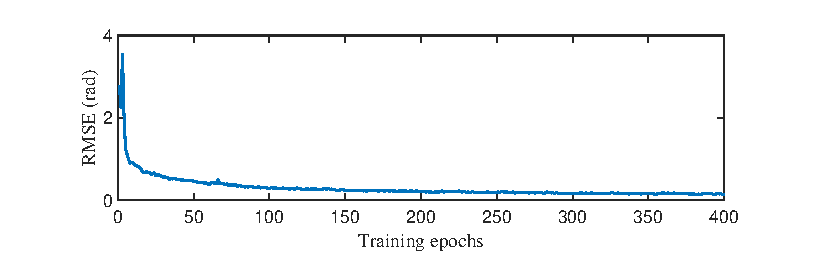
\includegraphics[scale=0.65]{results_rmse}
        \label{results_rmse}
        }
    \subfigure[Loss of the LSTM Network]{
        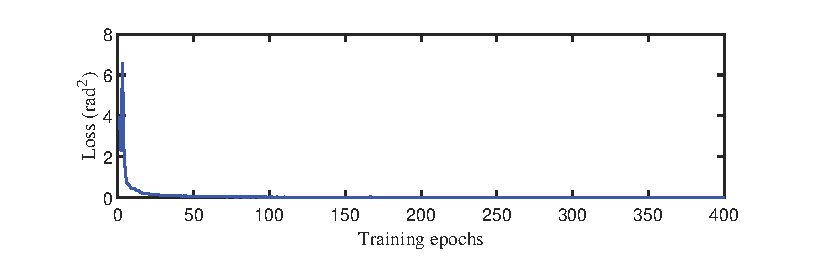
\includegraphics[scale=0.65]{results_loss}
        \label{results_loss}
    }
    \caption{Convergence of the LSTM network}
    \label{results_convergence}
\end{figure}

Fig.~\ref{results_convergence} demonstrates the convergence of the LSTM network.
The root-mean-square error (RMSE) of the LSTM network is shown in Fig.~\ref{results_rmse}.
It is observed that the RMSE rapidly converges to about $0.4$ around $50$th epoch, and finally converges to about $0.2$ after $400$ epochs.
And the loss of the LSTM network is shown in Fig.~\ref{results_loss}.
It shows that the loss decreases sharply around $20$ epochs, and finally converges to a small value about $0.01$ after $400$ epochs.

% 16 * 4 天线,不同噪声方差下的平均 SNR,中断次数和观测次数
% 随着噪声方差增大,平均 SNR 降低,中断次数和观测次数增多。
\begin{figure}[!t]
    \centering
    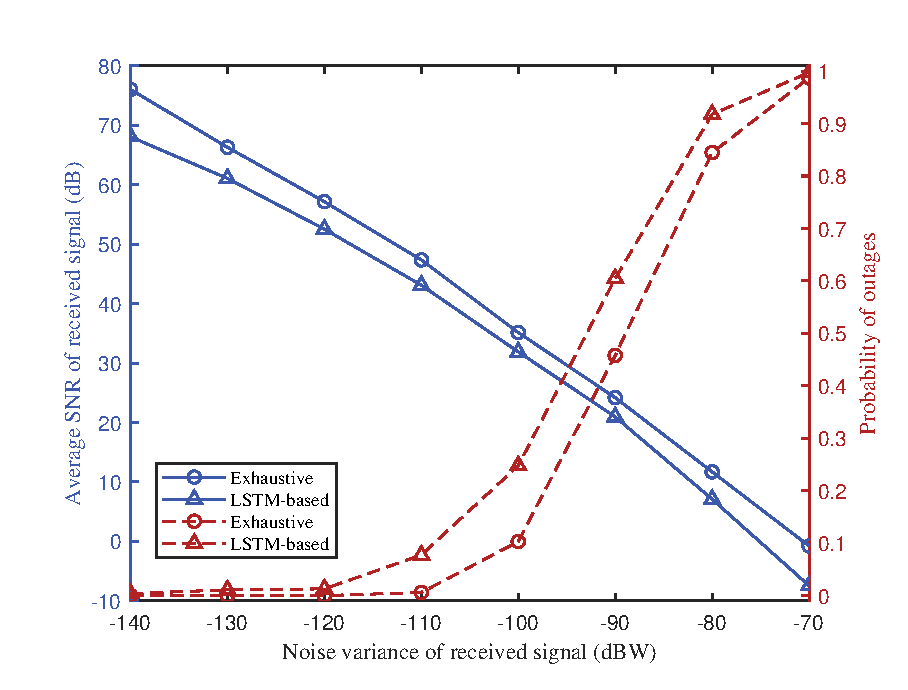
\includegraphics[scale=0.54]{results_noise}
    \caption{Average SNR and outages probability versus $\sigma_v^2$}
    \label{results_noise}
\end{figure}
Fig.~\ref{results_noise} shows the performance of schemes versus $\sigma_v^2$.
It is observed that for both exhaustive and FC-BET scheme, the average SNR of received signal decreases and the probability of outages increases with the increase of $\sigma_v^2$.
The difference in the average SNR between FC-BET scheme and exhaustive scheme is small, up to about $8$ dB.
When $\sigma_v^2=-120$ dBW, there is not any outage in exhaustive scheme, and the average SNR of received signal in exhaustive scheme is $57.16$ dB compared with $52.53$ dB in FC-BET scheme, with a loss of only $4.63$ dB in SNR, indicating a loss of about $8.1\%$ in spectral efficiency.

\begin{table}[!b]
    \newcommand{\tabincell}[2]{\begin{tabular}{@{}#1@{}}#2\end{tabular}}
    \renewcommand{\arraystretch}{1.3}
    \centering
    \begin{threeparttable}
    \caption{\label{t_NM}Measurement Overhead Comparisons of Various Schemes}
        \begin{tabular}{c c c}
            \hline
            \bfseries Schemes & \bfseries Complexity & \bfseries Measurement Overhead\\
            \hline
            FC-BET & $N_s + n_L 4 N_f M_r M_t$\tnote{1} & $13799$\\
            Hierarchical & $2 N log_2{4 M_r M_t}$ & $16144$\\ % $N (2 (\log_2{2 M_t} - \log_2{2 M_r}) + 4 \log_2{2 M_r})$
            Exhaustive & $4 N M_r M_t$ & $258304$\\
            \hline
        \end{tabular}
        \begin{tablenotes}
            \item[1] $N_s$ is the number of successful prediction and $N_f = N - N_s$.
        \end{tablenotes}
    \end{threeparttable}
\end{table}

Table \ref{t_NM} shows the comparison of measurement overhead in different schemes.
The proposed FC-BET scheme reduces the measurement overhead by about $98.3\%$ and $14.5\%$ compared with exhaustive and hierarchical schemes, respectively.
Considering the significant reduction in measurement overhead, the $8.1\%$ loss of spectral efficiency in Fig.~\ref{results_noise} seems acceptable.
Note that FC-BET scheme performs initial estimation for prediction by exhaustive search approach in this paper, and it is obvious that the measurement overhead can be further reduced by utilizing a smarter beam search approach.

\begin{table}[!t]
    \renewcommand{\arraystretch}{1.3}
    \caption{Performance and Overhead Comparisons of Different $n_L$}
    \label{t_LBC}
    \centering
    \begin{tabular}{c | c c c c c}
        \hline
        \bfseries Lookback $n_L$ & 1 & 3 & 5 & 10\\
        \hline
        \bfseries Average SNR (dB) & 52.98 & 49.56 & \bfseries 53.74 & 50.91\\
        \hline
        \bfseries Outage probability & 0.032 & 0.020 & 0.010 & \bfseries 0.009\\
        \hline
        \bfseries Measurement Overhead & \bfseries 9169 & 16349 & 13799 & 24040\\
        \hline
    \end{tabular}
\end{table}
% https://medium.com/@iamvarman/how-to-calculate-the-number-of-parameters-in-the-cnn-5bd55364d7ca
% https://stackoverflow.com/questions/38080035/how-to-calculate-the-number-of-parameters-of-an-lstm-network
% LSTM: num_params = [(num_units + input_dim + 1) * num_units] * 4
% Dropout: 0 
% Fully connected: (input_dim + 1) * output_dim

In FC-BET scheme, $n_L$ determines the number of beam searches in initial estimation and the length of feature in LSTM network.
The comparisons of performance with different $n_L$ are shown in Table \ref{t_LBC}.
It is observed that with the increase of $n_L$, the outage probability decreases.
However, counterintuitively, it seems that the SNR is independent with $n_L$.
A reasonable guess is that larger $n_L$ reduce the outage probability but increase the uncertainty of predictions, which leads to fluctuations in SNR.
On the other hand, larger $n_L$ introduces longer initial estimation which may result in more measurements, therefore trade-off between performance and overhead should be considered.

\begin{figure}[!t]
    \centering
    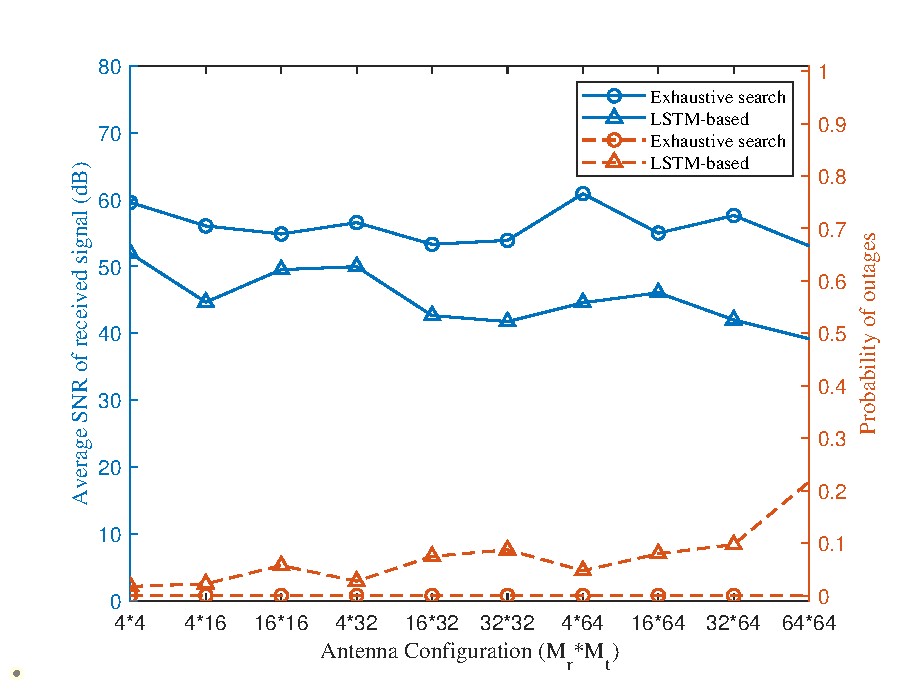
\includegraphics[scale=0.54]{results_antenna}
    \caption{Average SNR and outages probability versus $M_t \times M_r$}
    \label{results_antenna}
\end{figure}

Fig.~\ref{results_antenna} shows that the difference of performance between FC-BET and exhaustive scheme increase with the number of antennas.
The reason is that the beam widths of the vehicle and the BS become smaller when the number of antennas become bigger, thus reducing tolerance for beam deflection.
It is noteworthy that the slow increase in outage probability implies that it is possible for FC-BET scheme to be applied in massive MIMO with further improvements.

\section{Conclusions}\label{C}

This paper studies the beam tracking problem in mmWave vehicular communications with ULA.
A fast consecutive beam tracking scheme based on LSTM, called FC-BET, is proposed to reduce the beam training overhead in a common vehicular scenario.
In order to evaluate the proposed scheme, a time series channel dataset is built by statistical channel model using sequential vehicle information generated from SUMO.
Simulation results have verified the FC-BET scheme can reduce the measurement overhead by $98.3\%$ and $14.5\%$ compared with the exhaustive and hierarchical schemes, respectively, with a loss of about $8.1\%$ in spectral efficiency.

\section*{Acknowledgment}

This work was supported in part by the China Postdoctoral Science Foundation under Grant 2019M650587, and in part by the National Natural Science Foundation of China under Grant 61801047.
% This work was supported in part by the National Natural Science Foundation of China (00000000), in part by the Beijing Key Laboratory of Network System Architecture and Convergence and in part by Beijing Laboratory of Advanced Information Networks.

\bibliographystyle{IEEEtran}
\bibliography{references}

\end{document}